\documentclass{training}
\schoollogo{../../resources/intros/UX-00-athlete-keep-hydrated.jpg}
\newcommand{\uxfond}{../../resources/fond/UX-00-athlete-keep-hydrated.png}
% Filigrane PAR MODULE : \uxfond (PNG A4 dilue 30 %). Cadre noir vectoriel commun.
% Proportions original 744 px : marge 20/744, trait 1/744. Exterieur BLANC.
% Cadre via eso-pic +\put (coordonnees absolues) — pas de remember picture (decalage).
\usepackage{eso-pic}

\providecommand{\uxfond}{../../resources/fond/norme_fond_paliers_30.png}

\newlength{\uxmargin}
\newlength{\uxthick}
\newlength{\uxinnerw}
\newlength{\uxinnerh}
\setlength{\uxmargin}{0.02688\paperwidth}% 20/744
\setlength{\uxthick}{0.001344\paperwidth}% 1/744
\setlength{\uxinnerw}{\dimexpr\paperwidth-2\uxmargin-2\uxthick\relax}
\setlength{\uxinnerh}{\dimexpr\paperheight-2\uxmargin-2\uxthick\relax}

% Contenu strictement a l'interieur du trait (+ jour confortable).
\geometry{%
  includeheadfoot,
  left=22mm,
  right=22mm,
  top=20mm,
  bottom=18mm,
  headheight=30pt,
  headsep=5mm,
  footskip=12mm%
}

\AddToShipoutPictureBG{%
  \AtPageLowerLeft{%
    % Fond blanc page entiere
    \put(0,0){\color{white}\rule{\paperwidth}{\paperheight}}%
    % Filigrane module a l'interieur du cadre
    \put(\LenToUnit{\dimexpr\uxmargin+\uxthick\relax},\LenToUnit{\dimexpr\uxmargin+\uxthick\relax}){%
      \includegraphics[width=\uxinnerw,height=\uxinnerh]{\uxfond}}%
    % Cadre noir : bas, haut, gauche, droite
    \put(\LenToUnit{\uxmargin},\LenToUnit{\uxmargin}){%
      \color{black}\rule{\dimexpr\paperwidth-2\uxmargin\relax}{\uxthick}}%
    \put(\LenToUnit{\uxmargin},\LenToUnit{\dimexpr\paperheight-\uxmargin-\uxthick\relax}){%
      \color{black}\rule{\dimexpr\paperwidth-2\uxmargin\relax}{\uxthick}}%
    \put(\LenToUnit{\uxmargin},\LenToUnit{\uxmargin}){%
      \color{black}\rule{\uxthick}{\dimexpr\paperheight-2\uxmargin\relax}}%
    \put(\LenToUnit{\dimexpr\paperwidth-\uxmargin-\uxthick\relax},\LenToUnit{\uxmargin}){%
      \color{black}\rule{\uxthick}{\dimexpr\paperheight-2\uxmargin\relax}}%
  }%
}

\makeatletter
\fancyhf{}
\fancyheadoffset{0pt}
\renewcommand{\headrulewidth}{0pt}
\lhead{\parbox[t]{0.56\textwidth}{\RaggedRight\footnotesize\sloppy\@title}}
\rhead{\parbox[t]{0.36\textwidth}{\RaggedLeft\footnotesize\sloppy\@subtitle}}
\cfoot{\thepage}
% Coupures : underscore et slash dans les noms de fichiers / consignes
\DeclareRobustCommand{\_}{\textunderscore\allowbreak}
\makeatother

% Evite les depassements de longues lignes (Github, Name_FirstName_...)
\sloppy
\emergencystretch=3em
\hbadness=10000

% Sommaire type 42 : chapitres seulement
\setcounter{tocdepth}{0}
\renewcommand{\cftchappresnum}{}
\renewcommand{\cftchapaftersnum}{}
\setlength{\cftchapnumwidth}{2.0em}
\setlength{\cftbeforechapskip}{0.35em}
\cftsetindents{chapter}{0em}{2.0em}


\begin{document}

\title{Athlete, keep hydrated}
\subtitle{Piscine UX/UI --- UX}
\member{Piscine UX/UI}{https://github.com/01-edu/UX-UI}
\summary{A non-digital answer to how runners drink.}
\version{1.0}
\prerequisite{The previous module of this piscine, or none if this is your first.}
\maketitle

\newpage
\tableofcontents
\newpage


\chapter{Instructions}

The foreword is not an exercise. It will not be graded. The exercises start at the next chapter, from the easiest contract to the hardest. A later exercise is not taken into account if an earlier one does not hold.

Only what is in the turn-in directory of an exercise is looked at. Do not add files that the exercise does not name. The name of a deliverable follows the pattern in the exercise: \texttt{Name\_FirstName\_DeliverableName\_Date\_VersionNumber}.

You will not be given the gesture. The examples in an exercise sometimes carry a constraint that the sentence does not repeat. Read them. Your other references are the manual of the tool you picked, the person sitting next to you, and the links printed in the exercise.

The order is the order of the quest. Skipping a step because a later screen looks more interesting produces a screen nobody can explain.

\subsection*{About the pictures}

The mark on the cover is the picture of this module. The pale steps behind the text are the page ground. Neither one is a hint.

\subsection*{About machines that write}

You may use a tool to look up a term, the way you would use a dictionary. You may not replace an interview, a test, or a file with a generated text and sign it. If you cannot point at the person, the screen, or the line you claim, the exercise is not done.


\chapter{Foreword}

Before the screens, there is the road. \emph{Chariots of Fire} (Hugh Hudson, 1981) spends its time on two runners and almost none on the gadget that will save them. This quest is in that spirit: the hydration problem is real, and the answer you turn in does not have to be an application. The film does not tell you what to build. Neither does this page.

\begin{center}
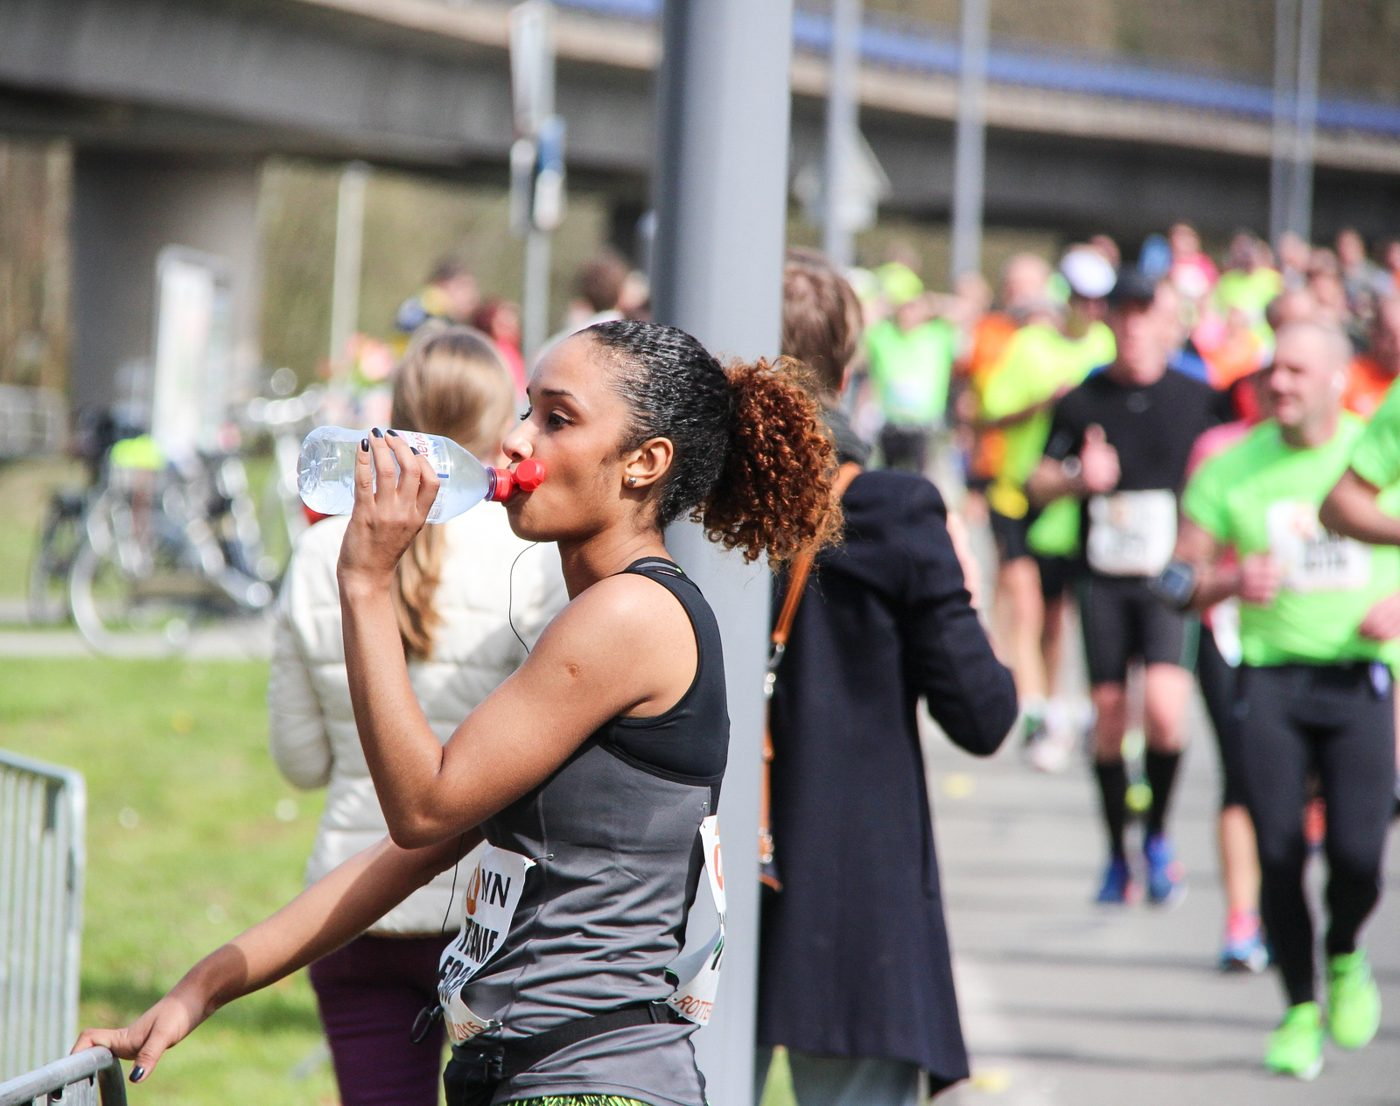
\includegraphics[width=0.78\textwidth,height=0.32\textheight,keepaspectratio]{../../resources/intros/UX-00-athlete-keep-hydrated.jpg}\\[0.4em]
{\footnotesize Picture: Peter van der Sluijs, CC BY-SA 3.0}
\end{center}

Recommended watching. The videos are context. They are not the deliverable.
\begin{itemize}
\item UX - Introduction \& Quest n°1, 01Edu \url{https://www.youtube.com/watch?v=UbE6WMeuvQg&list=PLHyAJ_GrRtf-RAtfngbRrFh1XDTnyXFDe}
\end{itemize}

\chapter{Exercise 00: UX I - Ex 1 - User Interviews}
\exnumber{00}
\extitle{UX I - Ex 1 - User Interviews}
\exfiles{ex00/PDF, named Name\_FirstName\_DeliverableName\_Date\_VersionNumber}
\exauthorize{Those named in the exercise}
\makeheaderfiles

\textbf{Context:}

Welcome to the very first quest of this program.

Your mission, should you choose to accept it, is to find a way to improve athletes' experience related to their hydration when running.

This first project is very special: you are asked to end up with a non-digital solution. As a matter of fact, innovation does not always rhyme with digital. So let's be creative and get out of the box!

\textbf{General recommendations:}

\begin{itemize}
\item Get Out of the Box. Be curious. Follow design trends on YouTube, LinkedIn, in podcasts, on Instagram accounts. Explore the internet when you discover a new concept. Build your own design culture.
\item Document everything you do, take notes, open a medium account to identify and show your deliverables, thoughts and feedback. It will be useful for your portoflio!
\item Trust the design process. One step after another.
\item Design needs to fail. 
\end{itemize}
Failure is even a necessary step, but ideally it should happen before a product is launched, during the prototype and test phases
\begin{itemize}
\item Make connections. Use LinkedIn, your friends, friends of friends to frequently meet designers and ask them about how they practice design in their organization. Who know, some day thay may remember you and offer you a contract!
\item Have fun!!
\end{itemize}

\textbf{Instructions:}

\begin{itemize}
\item Read all the scripts very carefully
\item Extract at least 6 insights and write them down on a PDF file
\begin{itemize}
\item Insights must be either shared by several people or consistent with what other people have already experienced
\item For each insight, name who said it.
\end{itemize}
\item Definition of 'insight': A key learning from what you have seen, read or heard. 
\end{itemize}

\textbf{Deliverables:}

\begin{itemize}
\item Create a PDF document and write at least 6 insights and the name of the person(s) who said it.
\item Upload the PDF document on Github, labeled as follows: "Name\_FirstName\_DeliverableName\_Date\_VersionNumber". For example, it can be labeled as "Doe\_John\_MidFiPrototype\_05242024\_V1".
\item Add a title within the document.
\item Pay attention to the global aspect of the document. It must be clear, simple and easy to read. You can get inspiration on canva.com but don't overload your design with too much details!
\end{itemize}

\textbf{Tips:}

\begin{itemize}
\item Examples of insights from the scripts (non-exhaustive list):
\begin{itemize}
\item Runs several times a week (Joe, Nathan, Guillaume, Anaelle)
\item Doesn't drink too much right before the race because it hurts my stomach (Nathan, Anaelle)
\item I run races with friends or peers (Joe, Nathan, Guillaume)
\end{itemize}
\end{itemize}

\begin{itemize}
\item The following is the interview script used to conduct the seven user interviews.
\item Interview guide:
\end{itemize}

Hello! My name is Agathe and I am conducting research about athletes and people who practice sports regularly. Hence, I'd be very happy to ask you some questions about the way you run, your habits, and the pain points you may have.

This interview will probably last 20 to 30 minutes.

Do you have any questions before we start?

Run

\begin{itemize}
\item What sports do you practice?
\item How often do you run?
\item When was the last time you went out for a run?
\end{itemize}

Races

\begin{itemize}
\item What was the last race you ran?
\item How was it? Tell me about the experience you had.
\item How did you get prepared?
\item What would you have done differently? Why?
\end{itemize}

Hydration

\begin{itemize}
\item What do you remember about the way you hydrated?
\item How did you manage your hydration?
\item Have you ever found yourself in trouble due to hydration? What happened?
\item What would you never do again? Why?
\end{itemize}

That's it, we went through all the questions I had.

Thank you so much for your time!

I have a last favor to ask you: is there anyone you know who runs frequently and would be available for a talk?


\chapter{Exercise 01: UX I - Ex 2 - Analytics}
\exnumber{01}
\extitle{UX I - Ex 2 - Analytics}
\exfiles{ex01/PDF, named Name\_FirstName\_DeliverableName\_Date\_VersionNumber}
\exauthorize{Those named in the exercise}
\makeheaderfiles

\textbf{Instructions:}

Read these articles and extract at least 5 key figures or insights that may be useful in understanding what athletes or sport practicing people experience related to hydration.

\textbf{Deliverables:}

\begin{itemize}
\item On a PDF document, write at least 5 key figures or insights you extracted from the articles. 
\end{itemize}
Each insight or key figure should be justified by a quote and the title of the article.
\begin{itemize}
\item Upload the document on Github, labeled as follows: "Name\_FirstName\_DeliverableName\_Date\_VersionNumber". For example, it can be labeled as "Doe\_John\_MidFiPrototype\_05242024\_V1".
\item Add a title within the document.
\item Pay attention to the global aspect of the document. It must be clear, simple and easy to read. You can get inspiration on canva.com but don't overload your design with too much details!
\end{itemize}

\textbf{Resources:}

\begin{itemize}
\item The effects of Hydration on Athletic Performance \url{https://sportscardiologybc.org/the-effects-of-hydration-on-athletic-performance/}
\item Dehydration and its effects on performance - Human Kinetics \url{https://us.humankinetics.com/blogs/excerpt/dehydration-and-its-effects-on-performance}
\item Accuracy of Urine Color to Detect Equal to or Greater Than 2\% Body Mass Loss in Men Journal of Athletic Training \url{https://www.ncbi.nlm.nih.gov/pmc/articles/PMC4741257/}
\item Fluid replacement for the physically active - Journal of Athletic Training \url{https://www.ncbi.nlm.nih.gov/pmc/articles/PMC5634236/}
\item The importance of hydration - Harvard School of Public Health \url{https://www.hsph.harvard.edu/news/hsph-in-the-news/the-importance-of-hydration/}
\item Fluids and hydration in prolonged endurance performance - Pubmed \url{https://pubmed.ncbi.nlm.nih.gov/15212747/}
\end{itemize}

\textbf{Tips:}

Examples of insights you can extract from the articles:

\begin{itemize}
\item Symptoms of dehydration can be headache, dizziness, nausea, lightheadedness, or fatigue.
\item People experience dehydration when they lose 2\% of their body mass loss (BML) in fluids/water/sweat.
\item Sweat helps the body to maintain optimal body temperature.
\item Sprint athletes are generally less concerned about the effects of dehydration than are endurance athletes.
\item Etc...
\end{itemize}

It's on you to find other and more!

\textbf{Quote:}

Always base your decisions on the data, not on your biases.


\chapter{Exercise 02: UX I - Ex 3 - Personas}
\exnumber{02}
\extitle{UX I - Ex 3 - Personas}
\exfiles{ex02/Figma file and PDF, named Name\_FirstName\_DeliverableName\_Date\_VersionNumber}
\exauthorize{Those named in the exercise}
\makeheaderfiles

\textbf{Instructions:}

\begin{itemize}
\item Create a user persona based on several users from the same category
\end{itemize}

\textbf{Deliverables:}

\begin{itemize}
\item A user persona on a PDF document
\item Upload the PDF document on Github, labeled as follows: "Name\_FirstName\_DeliverableName\_Date\_VersionNumber". For example, it can be labeled as "Doe\_John\_MidFiPrototype\_05242024\_V1".
\item Add a title within the document.
\item Pay attention to the global aspect of the document. It must be clear, simple and easy to read. You can get inspiration on canva.com but don't overload your design with too much details!
\end{itemize}

\textbf{Tips:}

\begin{itemize}
\item You may use Figma and extract a PDF document out of it.
\item Use the material you got from exercise 1.
\item Detect people who face the same kinds of problems and group them. 
\item When you find 2+ people who face the same kind of problem, you can merge their testimonials to create a persona. In this case, Joe, Nathan, Guillaume and Anaelle who run races from time to time (they have run at least one race in their life, but less than 3 times a year) and have faced dehydration problems. 
\item A persona is fictional: do not use one of your users' names, but a name that is consistent with your users' demographics and social group. In this case, we'll choose a man as 3 out of 4 are men, and Pierre as a first name so it's different (but consistent) from Joe's, Nathan's, Guillaume's and Anaelle's.
\item As to the age, average the ages of your selected users. In this case, 32 (Joe is 30, Nathan is 39, Guillaume is 30 and Anaelle is 29).
\item The persona has to be sport-oriented, as it is the context of this research. However, broader information, like the scan info (jobs, location, etc.) are more than welcome to give more context.
\end{itemize}

\textbf{Resources:}

\begin{itemize}
\item Make your persona great again \url{https://uxdesign.cc/personas-e60c1c06ead1}
\item Persona, journey maps, user flow, site map, OH MY! \url{https://uxdesign.cc/personas-journey-maps-site-maps-and-user-flows-oh-my-e71d044b4bcb}
\item Persona framework \url{https://miro.medium.com/max/1400/0*RbHfR6BHhhFIENNf}
\end{itemize}

\textbf{Quote:}

'Focus unswervingly, on the customer' Jesse Hertzberg | Former COO of Squarespace


\chapter{Exercise 03: UX I - Ex 4 - User Journey}
\exnumber{03}
\extitle{UX I - Ex 4 - User Journey}
\exfiles{ex03/Figma file, named Name\_FirstName\_DeliverableName\_Date\_VersionNumber}
\exauthorize{Those named in the exercise}
\makeheaderfiles

\textbf{Instructions:}

Based on your persona card, and the interview scripts, design Pierre's user journey.

\textbf{Deliverables:}

\begin{itemize}
\item A Figma file with Pierre's user journey.
\item Upload the Figma file on Github, labeled as follows: "Name\_FirstName\_DeliverableName\_Date\_VersionNumber". For example, it can be labeled as "Doe\_John\_MidFiPrototype\_05242024\_V1".
\item Add a title within the file.
\item Pay attention to the global aspect of the file. It must be clear, simple and easy to read. You can get inspiration on canva.com but don't overload your design with too much details!
\end{itemize}

\textbf{Tips:}

\begin{itemize}
\item You may use Figma.
\item Mix up some insights and details from the interview scripts to write a journey that is consistent with Pierre's personality.
\item You can, for instance, describe Pierre's first marathon. The first phase could be the preparation, the second phase the race itself, and the third one how he feels about the race when he has done it.
\item Break down the story step-by-step and define Pierre's actions.
\item Focus on each action and define Pierre's thoughts and main emotion among the list.
\item Adapt the line to Pierre's thoughts and emotions.
\item Define the opportunities to improve Pierre's overall experience every time you see a pain point.
\end{itemize}

\textbf{Resources:}

Most articles you'll find will be about user journeys or customer journeys. Keep in mind that you can adapt this methodology to any persona with any kind of situation or process, even at school, outside the school, in the digital world, etc.

\begin{itemize}
\item Tool: User Journey Mapping Template on Figma \url{https://www.figma.com/file/sXdUDoTXwItU7dyQYVkY1w/Tool---User-Journey-Map}
\item A Lean UX Customer Journey Map \url{https://uxdesign.cc/proto-journey-a-lean-ux-customer-journey-map-30ea3a241edc}
\item How to create a Customer Journey Map \url{https://www.youtube.com/watch?v=mSxpVRo3BLg}
\item Journey Mapping: How to build it \url{https://www.lucidchart.com/blog/how-to-build-customer-journey-maps}
\item Journey Mapping : Template on Figma \url{https://www.figma.com/file/5tittjiznRCWTNR2xI5FIT/Untitled?node-id=0%3A1}
\item Example \url{https://d2slcw3kip6qmk.cloudfront.net/marketing/blog/2017Q3/SEO-initiative-customer-journey-mapping/CustomerJourneyMap1.png}
\end{itemize}

\textbf{Quote:}

'It's about catching customers in the act, and providing highly relevant and highly contextual information' Paul Maritz | CEO Pivotal


\chapter{Exercise 04: UX I - Ex 5 - Problem Statement}
\exnumber{04}
\extitle{UX I - Ex 5 - Problem Statement}
\exfiles{ex04/PDF, named Name\_FirstName\_DeliverableName\_Date\_VersionNumber}
\exauthorize{Those named in the exercise}
\makeheaderfiles

\textbf{Instructions:}

Based on the insights from the analytics and user interviews, comment the scope of possible problem statements.

\textbf{Deliverables:}

\begin{itemize}
\item On a PDF document, write down one problem statement that summarizes the main problem that Pierre has when he runs.
\item Upload the PDF document on Github, labeled as follows: "Name\_FirstName\_DeliverableName\_Date\_VersionNumber". For example, it can be labeled as "Doe\_John\_MidFiPrototype\_05242024\_V1".
\item Add a title within the document.
\item Pay attention to the global aspect of the document. It must be clear, simple and easy to read. You can get inspiration on canva.com but don't overload your design with too much details!
\end{itemize}

\textbf{Tips:}

\begin{itemize}
\item At this stage, it's important to focus on the problem, not on the solution! You can start tackling the problem after (re)defining it.
\item Several problem statements can be possible for each persona and user journey, but for this exercise, we are guiding you towards one.
\item Examples of correct problem statements: 
\begin{itemize}
\item How might we help Pierre (or your persona) measure and prepare his hydration before a race?
\item How might we make sure Pierre doesn't get dehydrated?
\item How might we make sure Pierre drinks the cups that are offered during the race?
\item How might we provide Pierre some drink that contains everything he needs to avoid dehydration?
\item How might make sure Pierre doesn't get drunk the night before the race?
\end{itemize}
\item Examples of wrong problem statements: 
\begin{itemize}
\item How might we make sure Pierre doesn't get dehydrated?
\begin{itemize}
\item Too broad  --- > The problem statement is out of the scope of running, so the solutions cannot be integrated in the specific context of running.
\end{itemize}
\item How might we make sure Pierre drinks the cups that are offered during the race?
\begin{itemize}
\item Too narrow  --- > There are plenty of options to avoid dehydration without drinking the cups that are offered during the race.
\end{itemize}
\item How might we provide Pierre with a drink that contains everything he needs to avoid dehydration?
\begin{itemize}
\item Focused on the solution, not the problem  --- > The problem statement is supposed to rephrase the brief and take into account the insights from the previous phase.
\end{itemize}
\item How might make sure Pierre doesn't get drunk the night before the race?
\begin{itemize}
\item Out of scope  --- > This is not about dehydration, nor about running.
\end{itemize}
\end{itemize}
\end{itemize}

\textbf{Resources:}

\begin{itemize}
\item Stuck on a problem? Just ask how might we \url{https://relab.academy/design-thinking/stuck-on-a-problem-just-ask-how-might-we/}
\item Problem statement \url{https://www.indeed.com/career-advice/career-development/what-is-a-problem-statement}
\item Using 'How Might We' Questions to Ideative on the Right Problems \url{https://www.nngroup.com/articles/how-might-we-questions/}
\end{itemize}

\textbf{Quote:}

"If I had an hour to solve a problem, I'd spend 55 minutes thinking about the problem and 5 minutes thinking about solutions." Albert Einstein


\chapter{Exercise 05: UX I - Ex 6 - Ideation}
\exnumber{05}
\extitle{UX I - Ex 6 - Ideation}
\exfiles{ex05/Figma file and PDF, named Name\_FirstName\_DeliverableName\_Date\_VersionNumber}
\exauthorize{Those named in the exercise}
\makeheaderfiles

\textbf{Instructions:}

\emph{You can replace Pierre with your own persona.}

The chosen problem statement is: "How might we help Pierre (or your persona) measure and prepare his hydration before a race?"

Now, let's find creative solutions! Remember, the solution should not be digital! Forget about devices for this quest ;)

Find 3 friends outside of the program and run a quick ideation session (20 minutes).

\begin{itemize}
\item What you need for an in-person ideation workshop:
\begin{itemize}
\item Prepare some papers or sticky notes, stickers, a jar, and pens.
\item A closed room for 20 minutes where everyone feels comfortable
\end{itemize}
\item Directions:
\begin{itemize}
\item Ask them to turn off their phones
\item Explain the context and introduce Pierre (or your persona)
\item Explain the goal:
\begin{itemize}
\item Let's find as many solutions as possible to the question: "How might we help Pierre (or your persona) measure and prepare his hydration before a race?", given the following contraints (unveil them one after the other: 1 minute per constraint, 1 constraint per round):
\begin{itemize}
\item If Pierre was blind
\item If Pierre was a bird
\item If Pierre was a billionaire
\item If Pierre had a twin who was constantly with him
\item If Pierre was 5 years old
\item If Pierre had 5 arms
\item If Pierre was 105 years old
\item If Pierre was very clumsy
\item If Pierre was very forgetful (and lost memory every 5 minutes)
\item If Pierre was deaf
\item If Pierre was a turtle
\item If Pierre was naked
\item If Pierre couldn't stop talking 24/7
\item If Pierre was always late
\item If Pierre was dishonest
\end{itemize}
\end{itemize}
\item Set a timer for each round.
\item Ask the participants to do, at each round, the following:
\begin{itemize}
\item Write down their ideas on a sticky note (1 idea per sticky note)
\item Read them out loud
\item Put the sticky note in a jar
\end{itemize}
\item Gather all the ideas.
\item Give the participants 3 stickers each and ask them to vote for the best three options.
\item If there isn't a solution that stands out of the crowd, hang them on a board and organize them according to these two parameters: easy to implement and efficient. Example in the resources.
\item Choose 1 main idea to solve the problem
\end{itemize}
\end{itemize}

\textbf{Deliverables:}

\begin{itemize}
\item Pictures of the session
\item A board with all the ideas (on paper or digitally on Miro or Figma)
\item One main idea to solve the problem next to the board
\item Upload the documents on Github, in a zip folder named "ProjectTitle\_Name\_FirstName", with all project deliverables as follows: "Name\_FirstName\_DeliverableName\_Date\_VersionNumber".  For example, the first deliverable can be named as "Doe\_John\_MidFiPrototype\_05242024\_V1".
\item Add a title within all written documents.
\item Pay attention to the global aspect of the deliverables. They must be clear, simple and easy to read. You can get inspiration on canva.com but don't overload your design with too much details!
\end{itemize}

\textbf{Resources:}

\begin{itemize}
\item Tool: Ideation Voting Board Framework on Figma \url{https://www.figma.com/file/nTAWiacCffXvd8dXsLP3Sb/Ideation-Voting-Framework}
\item Where Good ideas come from by Steven Johnson \url{https://www.ted.com/talks/steven_johnson_where_good_ideas_come_from}
\item Creative Confidence by Tom Keller \url{https://booksvooks.com/creative-confidence-unleashing-the-creative-potential-within-us-all-pdf.html}
\item Podcast What is wrong with UX? \url{https://www.usersknow.com/podcast/2016/10/10/ua1wdsszhx2pemugxc1e0qj0a3l9cs}
\item Brainwriting \#2 \url{https://dux.typepad.com/dux/2011/01/method-2-of-100-brainwriting-brainwriting-is-an-ideation-method-for-quickly-generating-ideas-by-asking-people-to-write-thei.html}
\end{itemize}

\textbf{Quote:}

Chances are that... If you have gone through all possible solutions, you've found the good one.


\chapter{Exercise 06: UX I - Ex 7 - Prototyping}
\exnumber{06}
\extitle{UX I - Ex 7 - Prototyping}
\exfiles{ex06/zip archive, named Name\_FirstName\_DeliverableName\_Date\_VersionNumber}
\exauthorize{Those named in the exercise}
\makeheaderfiles

\textbf{Instructions:}

Develop your idea!

Design a storyboard of Pierre (or your persona) using your idea as a solution. Show all the steps (from 6 to 12) with drawings on paper.

\textbf{Deliverables:}

\begin{itemize}
\item Pictures of 1 storyboard to describe your solution, on paper
\item Upload the documents on Github, in a zip folder named "ProjectTitle\_Name\_FirstName", with all project deliverables as follows: "Name\_FirstName\_DeliverableName\_Date\_VersionNumber".  For example, the first deliverable can be named as "Doe\_John\_MidFiPrototype\_05242024\_V1".
\item Add a title within all written documents.
\item Pay attention to the global aspect of the deliverables. They must be clear, simple and easy to read. You can get inspiration on canva.com but don't overload your design with too much details!
\end{itemize}

\textbf{Tips:}

\begin{itemize}
\item 1 drawing per action
\end{itemize}

\textbf{Resources:}

\begin{itemize}
\item How UX storyboards can transform your creative process \url{https://uxdesign.cc/ux-storyboarding-2ce43875f3de?sk=41b28ecef8c52d9944e5e636881111cf}
\item 17 reasons to use storyboards in UX design \url{https://uxdesign.cc/17-reasons-to-use-a-storyboards-in-ux-design-2bc6fea73e20?source=friends_link&sk=5bb2722f1f9ff06d4f22b0abfe52f508}
\item How to storyboard experiences \url{https://uxdesign.cc/how-to-storyboard-experiences-fc051e2bc04d}
\item Using comic strips and storyboards to test your UX concepts \url{https://uxdesign.cc/using-comic-strips-and-storyboards-to-test-your-ux-concepts-cccad7ac7f71}
\end{itemize}

\textbf{Quote:}

"No product is an island. A product is more than the product. It is a cohesive, integrated set of experiences" Don Norman


\end{document}
